\documentclass[twocolumn,11pts]{IEEEtran}
% packages to make the language spanish
\usepackage[spanish,es-lcroman,es-tabla,es-nosectiondot]{babel}
\decimalpoint% changes the coma in the numbers to period
\usepackage[utf8]{inputenc}
\usepackage[T1]{fontenc}
\usepackage{csquotes}
\usepackage{graphicx}

% Some very useful LaTeX packages include:
% (uncomment the ones you want to load)

% *** CAPTION ***
\usepackage[font=footnotesize,labelfont=bf,labelsep=period]{caption}

% *** CITATION PACKAGES ***
%
\usepackage{cite}
%
% cite.sty was written by Donald Arseneau
% V1.6 and later of IEEEtran pre-defines the format of the cite.sty package
% \cite{} output to follow that of IEEE. Loading the cite package will
% result in citation numbers being automatically sorted and properly
% "compressed/ranged". e.g., [1], [9], [2], [7], [5], [6] without using
% cite.sty will become [1], [2], [5]--[7], [9] using cite.sty. cite.sty's
% \cite will automatically add leading space, if needed. Use cite.sty's
% noadjust option (cite.sty V3.8 and later) if you want to turn this off.
% cite.sty is already installed on most LaTeX systems. Be sure and use
% version 4.0 (2003-05-27) and later if using hyperref.sty. cite.sty does
% not currently provide for hyperlinked citations.
% The latest version can be obtained at:
% http://www.ctan.org/tex-archive/macros/latex/contrib/cite/
% The documentation is contained in the cite.sty file itself.

% Bibliografia para este documento
% Se incluye embebida para poder transportarla en el mismo documento. Sin embargo,
% en sus documentos puede tener esta información en el archivo *.bib.
% Consecuentemente, no necesita el uso del paquete filecontents.
\usepackage{filecontents}
\begin{filecontents}{guia.bib}
% note el uso de las llaves {} para escapar la instrucción \LaTeX dentro del título del artículo
@ARTICLE{Downes2002,
  title = {Short Math Guide for {\LaTeX}},
  author = {Michael Downes},
  year = {2002},
  url = {ftp://ftp.ams.org/pub/tex/doc/amsmath/short-math-guide.pdf}
}
\end{filecontents}


% *** GRAPHICS RELATED PACKAGES ***
%
% \usepackage[pdftex]{graphicx}
% declare the path(s) where your graphic files are
% \graphicspath{{../pdf/}{../jpeg/}}
% and their extensions so you won't have to specify these with
% every instance of \includegraphics
% \DeclareGraphicsExtensions{.pdf,.jpeg,.png}
%
% graphicx was written by David Carlisle and Sebastian Rahtz. It is
% required if you want graphics, photos, etc. graphicx.sty is already
% installed on most LaTeX systems. The latest version and documentation can
% be obtained at: 
% http://www.ctan.org/tex-archive/macros/latex/required/graphics/
% Another good source of documentation is "Using Imported Graphics in
% LaTeX2e" by Keith Reckdahl which can be found as epslatex.ps or
% epslatex.pdf at: http://www.ctan.org/tex-archive/info/
%
% latex, and pdflatex in dvi mode, support graphics in encapsulated
% postscript (.eps) format. pdflatex in pdf mode supports graphics
% in .pdf, .jpeg, .png and .mps (metapost) formats. Users should ensure
% that all non-photo figures use a vector format (.eps, .pdf, .mps) and
% not a bitmapped formats (.jpeg, .png). IEEE frowns on bitmapped formats
% which can result in "jaggedy"/blurry rendering of lines and letters as
% well as large increases in file sizes.
%
% You can find documentation about the pdfTeX application at:
% http://www.tug.org/applications/pdftex


% *** MATH PACKAGES ***
%
%\usepackage[cmex10]{amsmath}
% A popular package from the American Mathematical Society that provides
% many useful and powerful commands for dealing with mathematics. If using
% it, be sure to load this package with the cmex10 option to ensure that
% only type 1 fonts will utilized at all point sizes. Without this option,
% it is possible that some math symbols, particularly those within
% footnotes, will be rendered in bitmap form which will result in a
% document that can not be IEEE Xplore compliant!
%
% Also, note that the amsmath package sets \interdisplaylinepenalty to 10000
% thus preventing page breaks from occurring within multiline equations. Use:
%\interdisplaylinepenalty=2500
% after loading amsmath to restore such page breaks as IEEEtran.cls normally
% does. amsmath.sty is already installed on most LaTeX systems. The latest
% version and documentation can be obtained at:
% http://www.ctan.org/tex-archive/macros/latex/required/amslatex/math/


% *** SPECIALIZED LIST PACKAGES ***
%
\usepackage{algorithm}
\usepackage{algpseudocode}
\makeatletter
\renewcommand{\ALG@name}{Algoritmo}% Algorithm -> Algoritmo
\makeatother
\captionsetup[algorithm]{font=footnotesize,labelsep=period}
% algorithmic.sty was written by Peter Williams and Rogerio Brito.
% This package provides an algorithmic environment fo describing algorithms.
% You can use the algorithmic environment in-text or within a figure
% environment to provide for a floating algorithm. Do NOT use the algorithm
% floating environment provided by algorithm.sty (by the same authors) or
% algorithm2e.sty (by Christophe Fiorio) as IEEE does not use dedicated
% algorithm float types and packages that provide these will not provide
% correct IEEE style captions. The latest version and documentation of
% algorithmic.sty can be obtained at:
% http://www.ctan.org/tex-archive/macros/latex/contrib/algorithms/
% There is also a support site at:
% http://algorithms.berlios.de/index.html
% Also of interest may be the (relatively newer and more customizable)
% algorithmicx.sty package by Szasz Janos:
% http://www.ctan.org/tex-archive/macros/latex/contrib/algorithmicx/

\usepackage{listings}
\usepackage{tikz}
\lstset{
  language=[LaTeX]TeX,
  breaklines=true,
  basicstyle=\tt\scriptsize,
  keywordstyle=\color{blue},
  identifierstyle=\color{magenta},
  commentstyle=\color{green!40!black},
  % frame 
  frame=tb,
  captionpos=t,
  xleftmargin=1em,
  numbersep=0.3em,
  numbers=left,
  framexleftmargin=1.1em,
  framexrightmargin=0pt,
  % additional letters for accents in spanish
  literate=%
    {á}{{\'{a}}}1
    {é}{{\'{e}}}1
    {í}{{\'{i}}}1
    {ó}{{\'{o}}}1
    {ú}{{\'{u}}}1
    {ñ}{{\~{n}}}1
    {Ñ}{{\~{N}}}1
}

\renewcommand{\lstlistingname}{Código}% Listing -> Código
\DeclareCaptionFormat{listing}{\rule{\dimexpr\linewidth\relax}{0.4pt}\par\vskip1pt#1#2#3}
\captionsetup[lstlisting]{format=listing,singlelinecheck=false, margin=0pt,position=bottom}

% *** ALIGNMENT PACKAGES ***
%
%\usepackage{array}
% Frank Mittelbach's and David Carlisle's array.sty patches and improves
% the standard LaTeX2e array and tabular environments to provide better
% appearance and additional user controls. As the default LaTeX2e table
% generation code is lacking to the point of almost being broken with
% respect to the quality of the end results, all users are strongly
% advised to use an enhanced (at the very least that provided by array.sty)
% set of table tools. array.sty is already installed on most systems. The
% latest version and documentation can be obtained at:
% http://www.ctan.org/tex-archive/macros/latex/required/tools/


%\usepackage{mdwmath}
%\usepackage{mdwtab}
% Also highly recommended is Mark Wooding's extremely powerful MDW tools,
% especially mdwmath.sty and mdwtab.sty which are used to format equations
% and tables, respectively. The MDWtools set is already installed on most
% LaTeX systems. The lastest version and documentation is available at:
% http://www.ctan.org/tex-archive/macros/latex/contrib/mdwtools/


% IEEEtran contains the IEEEeqnarray family of commands that can be used to
% generate multiline equations as well as matrices, tables, etc., of high
% quality.


%\usepackage{eqparbox}
% Also of notable interest is Scott Pakin's eqparbox package for creating
% (automatically sized) equal width boxes - aka "natural width parboxes".
% Available at:
% http://www.ctan.org/tex-archive/macros/latex/contrib/eqparbox/


% *** SUBFIGURE PACKAGES ***
%\usepackage[tight,footnotesize]{subfigure}
% subfigure.sty was written by Steven Douglas Cochran. This package makes it
% easy to put subfigures in your figures. e.g., "Figure 1a and 1b". For IEEE
% work, it is a good idea to load it with the tight package option to reduce
% the amount of white space around the subfigures. subfigure.sty is already
% installed on most LaTeX systems. The latest version and documentation can
% be obtained at:
% http://www.ctan.org/tex-archive/obsolete/macros/latex/contrib/subfigure/
% subfigure.sty has been superceeded by subfig.sty.


%\usepackage[caption=false]{caption}
%\usepackage[font=footnotesize]{subfig}
% subfig.sty, also written by Steven Douglas Cochran, is the modern
% replacement for subfigure.sty. However, subfig.sty requires and
% automatically loads Axel Sommerfeldt's caption.sty which will override
% IEEEtran.cls handling of captions and this will result in nonIEEE style
% figure/table captions. To prevent this problem, be sure and preload
% caption.sty with its "caption=false" package option. This is will preserve
% IEEEtran.cls handing of captions. Version 1.3 (2005/06/28) and later 
% (recommended due to many improvements over 1.2) of subfig.sty supports
% the caption=false option directly:
\usepackage[caption=false,font=footnotesize]{subfig}
%
% The latest version and documentation can be obtained at:
% http://www.ctan.org/tex-archive/macros/latex/contrib/subfig/
% The latest version and documentation of caption.sty can be obtained at:
% http://www.ctan.org/tex-archive/macros/latex/contrib/caption/


% *** FLOAT PACKAGES ***
%
%\usepackage{fixltx2e}
% fixltx2e, the successor to the earlier fix2col.sty, was written by
% Frank Mittelbach and David Carlisle. This package corrects a few problems
% in the LaTeX2e kernel, the most notable of which is that in current
% LaTeX2e releases, the ordering of single and double column floats is not
% guaranteed to be preserved. Thus, an unpatched LaTeX2e can allow a
% single column figure to be placed prior to an earlier double column
% figure. The latest version and documentation can be found at:
% http://www.ctan.org/tex-archive/macros/latex/base/

%\usepackage{stfloats}
% stfloats.sty was written by Sigitas Tolusis. This package gives LaTeX2e
% the ability to do double column floats at the bottom of the page as well
% as the top. (e.g., "\begin{figure*}[!b]" is not normally possible in
% LaTeX2e). It also provides a command:
%\fnbelowfloat
% to enable the placement of footnotes below bottom floats (the standard
% LaTeX2e kernel puts them above bottom floats). This is an invasive package
% which rewrites many portions of the LaTeX2e float routines. It may not work
% with other packages that modify the LaTeX2e float routines. The latest
% version and documentation can be obtained at:
% http://www.ctan.org/tex-archive/macros/latex/contrib/sttools/
% Documentation is contained in the stfloats.sty comments as well as in the
% presfull.pdf file. Do not use the stfloats baselinefloat ability as IEEE
% does not allow \baselineskip to stretch. Authors submitting work to the
% IEEE should note that IEEE rarely uses double column equations and
% that authors should try to avoid such use. Do not be tempted to use the
% cuted.sty or midfloat.sty packages (also by Sigitas Tolusis) as IEEE does
% not format its papers in such ways.

%\ifCLASSOPTIONcaptionsoff
%  \usepackage[nomarkers]{endfloat}
% \let\MYoriglatexcaption\caption
% \renewcommand{\caption}[2][\relax]{\MYoriglatexcaption[#2]{#2}}
%\fi
% endfloat.sty was written by James Darrell McCauley and Jeff Goldberg.
% This package may be useful when used in conjunction with IEEEtran.cls'
% captionsoff option. Some IEEE journals/societies require that submissions
% have lists of figures/tables at the end of the paper and that
% figures/tables without any captions are placed on a page by themselves at
% the end of the document. If needed, the draftcls IEEEtran class option or
% \CLASSINPUTbaselinestretch interface can be used to increase the line
% spacing as well. Be sure and use the nomarkers option of endfloat to
% prevent endfloat from "marking" where the figures would have been placed
% in the text. The two hack lines of code above are a slight modification of
% that suggested by in the endfloat docs (section 8.3.1) to ensure that
% the full captions always appear in the list of figures/tables - even if
% the user used the short optional argument of \caption[]{}.
% IEEE papers do not typically make use of \caption[]'s optional argument,
% so this should not be an issue. A similar trick can be used to disable
% captions of packages such as subfig.sty that lack options to turn off
% the subcaptions:
% For subfig.sty:
% \let\MYorigsubfloat\subfloat
% \renewcommand{\subfloat}[2][\relax]{\MYorigsubfloat[]{#2}}
% For subfigure.sty:
% \let\MYorigsubfigure\subfigure
% \renewcommand{\subfigure}[2][\relax]{\MYorigsubfigure[]{#2}}
% However, the above trick will not work if both optional arguments of
% the \subfloat/subfig command are used. Furthermore, there needs to be a
% description of each subfigure *somewhere* and endfloat does not add
% subfigure captions to its list of figures. Thus, the best approach is to
% avoid the use of subfigure captions (many IEEE journals avoid them anyway)
% and instead reference/explain all the subfigures within the main caption.
% The latest version of endfloat.sty and its documentation can obtained at:
% http://www.ctan.org/tex-archive/macros/latex/contrib/endfloat/
%
% The IEEEtran \ifCLASSOPTIONcaptionsoff conditional can also be used
% later in the document, say, to conditionally put the References on a 
% page by themselves.


% *** PDF, URL AND HYPERLINK PACKAGES ***
%
\usepackage{url}
% url.sty was written by Donald Arseneau. It provides better support for
% handling and breaking URLs. url.sty is already installed on most LaTeX
% systems. The latest version can be obtained at:
% http://www.ctan.org/tex-archive/macros/latex/contrib/misc/
% Read the url.sty source comments for usage information. Basically,
% \url{my_url_here}.

% *** Do not adjust lengths that control margins, column widths, etc. ***
% *** Do not use packages that alter fonts (such as pslatex).         ***
% There should be no need to do such things with IEEEtran.cls V1.6 and later.
% (Unless specifically asked to do so by the journal or conference you plan
% to submit to, of course. )

% this should be the latest package to load (unless you find an exception or 
% clash between packages)
\usepackage{hyperref}
\hypersetup{
  colorlinks=false,       % false: boxed links; true: colored links
  pdfborder={0 0 0}       % remove ugly border from links
}

% correct bad hyphenation here
\hyphenation{op-tical net-works semi-conduc-tor}

\begin{document}
% Patch for the \label command on showexpl
\let\orilabel\label

%
% paper title
% can use linebreaks \\ within to get better formatting as desired
\title{Sistema de voactión por reconocimiento automático}
%

\author{Daniel Méndez - Felipe Rios - Carlos Martínez - Luis Cáceres
%\thanks{Escuela de Informática y Telecomunicaciones}% <-this % stops a space
%\thanks{e-mail: adin.ramirez@mail.udp.cl.}% <-this % stops a space
}
% note the % following \thanks
% these prevent an unwanted space from occurring between the last author name
% and the end of the author line. i.e., if you had this:
% 
% \author{....lastname \thanks{...} \thanks{...} }
%                     ^------------^------------^----Do not want these spaces!
%
% a space would be appended to the last name and could cause every name on that
% line to be shifted left slightly. This is one of those "LaTeX things". For
% instance, "\textbf{A} \textbf{B}" will typeset as "A B" not "AB". To get
% "AB" then you have to do: "\textbf{A}\textbf{B}"
% \thanks is no different in this regard, so shield the last } of each \thanks
% that ends a line with a % and do not let a space in before the next \thanks.
% Spaces after \IEEEmembership other than the last one are OK (and needed) as
% you are supposed to have spaces between the names. For what it is worth,
% this is a minor point as most people would not even notice if the said evil
% space somehow managed to creep in.


% The paper headers
\markboth{Escuela de Informática y Telecomunicaciones}%
{Informe}%<- this part will appear only with the twoside option in the documentclass
% The only time the second header will appear is for the odd numbered pages
% after the title page when using the twoside option.

% make the title area
\maketitle


\begin{abstract}
La idea de este documento es dejar especificado los requerimientos, el análisis y diseño de los que se nos pide  y fijar una planificación de las metas a cumplir cada semana, hasta la fecha de entrega del producto final. Para esto debemos obtener, analizar, documentar, verificar y validar los requisitos del cliente. En base a diagramas lograr una estructura a desarrollar para poder realizar la plataforma tal como fue pedida.
\end{abstract}

\section{Introducción}

En una primera instancia se dió la opción de decidir entre 4 proyectos distintos, pero con un enfoque claro en la recopilación de datos por medio de cámaras, los cuales se analizaron detalladamente para decidir cual desarrollar, considerando el tiempo que tenemos, la composición del grupo y los gusto de cada integrante. Se eligió la opción que consiste en el conteo de votos automático a mano alzada, el cual puede ser anónimo o no. 

Esta elección se ve basada en la necedidad que tiene un profesor de identificar el aprendizaje de los alumnos en instancias anteriores a controles y solemnes, para así poder enfocar la clase y reforzar en los contenidos más debiles. Las herramientas que  existen para este acometido son escasas y poco usadas en nuestro entorno universitario, por esto queremos acercar y proveer de un sistema de opinión sencillo y fácil de usar, con la esperanza que sea usado en la universidad.

\section{Requerimientos}

\subsection{Visión General}
Planteamos desarrollar una herramienta que permita, a través de la camara ubicada en el laboratorio de informática, hacer encuestas y obtener las respuestas en tiempo real, detectando las manos alzadas de los alumnos, ya sea de manera anónima o con identificación y presentar los resultados de forma automática, el contador de votos y el detalle de estos. Además, se debe poder realizar preguntas, de una manera sencilla y facil de usar, para poder medir el aprendizaje de los alumnos en la sala.

\subsection{Requerimientos funcionales (RF)}
La tabla \ref{tabla1} muestra los requerimientos funcionales del proyecto.

\begin{table}[H]
\caption{Requerimientos funcionales.}
\label{tabla1}
\begin{center}
{\tt
\begin{tabular}{|c|c|c|}\hline
C\'odigo &Nombre &Descripci\'on \\\hline \hline
RF1 &Diferenciar personas & El sistema es capaz  \\ 
						& & de diferenciar una  \\ 
						& & persona de cualquier \\ 
						& & otro objeto presente \\
						& & en la sala. \\\hline
RF2 &Identificar personas & El sistema es capaz  \\ 
						& & de identificar una  \\ 
						& & persona desde una \\ 
						& & base de datos.\\\hline
RF3 &Distinguir mano alzada& Lograr diferenciar  \\ 
						& & cuando hay una mano  \\ 
						& & alzada dentro de  \\ 
						& & la sala.\\\hline
RF4 &Asignar mano alzada& Reconocer a que \\ 
						& & persona pertenece  \\ 
						& & la mano levantada. \\\hline	
RF5 &Contar cantidad manos& El sistema discrimina  \\ 
						& & si una persona \\ 
						& & levanta ambas manos. \\\hline	
RF6 &Contar votos & Contar cuantas personas  \\ 
						& & hicieron una votación. \\\hline										

\end{tabular}
}
\end{center}
\end{table}

\subsection{Requerimientos no funcionales (RNF)}

 La tabla \ref{tabla2} muestra los requerimientos no funcionales del proyecto.

\begin{table}[H]
\caption{Requerimientos no funcionales.}
\label{tabla2}
\begin{center}
{\tt
\begin{tabular}{|c|c|c|}\hline
C\'odigo &Nombre &Descripci\'on \\\hline \hline
RNF1 &Hacer encuesta& Se le permite al  \\ 
						& & usuario crear una  \\ 
						& & encuesta o pregunta \\ 
						& & para ser respondida.\\\hline
RNF2 &Ingresar alternativas &El usuario ingresa  \\ 
						& & las alternativas que  \\ 
						& & se pondrán a elección.\\\hline
RNF3 &Recopilar respuestas& Por cada alternativa  \\ 
						& & se recogen los datos  \\ 
						& & observados por la   \\ 
						& & cámara.\\\hline
RNF4 &Analizar resultados& Procesar los datos \\ 
						& & que se recogieron  \\ 
						& & para identificar los \\
						& & aciertos y errores. \\\hline	
RNF5 &Mostrar resultados& Mostrar gráficas\\ 
						& & de los datos analizados.\\\hline	
								

\end{tabular}
}
\end{center}
\end{table}

\section{Análisis}

La cámara captura imágenes por cuadros, los cuales son analizados y comparados para determinar si hay cambios dentro de la visual de esta y contrastar esa detección de movimiento contra el fondo estático reconocido como fondo de antemano.

Al recopilar la información obtenida por la cámara, se compararán ciertos espacios en la imágen demarcados por recuadros ubicados estrategicamente de manera tal que localizará una mano alzada ante una votación propuesta o note la presencia de una persona sin haber alzado su mano. 

Dentro de estos cuadros se verán las manos alzadas por los votantes y se hará un conteo de manos que aparezcan en los cuadros vs las manos que no aparezcan, se registrará este conteo y guardará la información de forma que el encuestador pueda ver la diferencia de votos a favor y en contra. Todo este proceso se llevará a cabo como se muestra en el siguiente diagrama de casos de uso.

\begin{figure}[H]
  \centering
  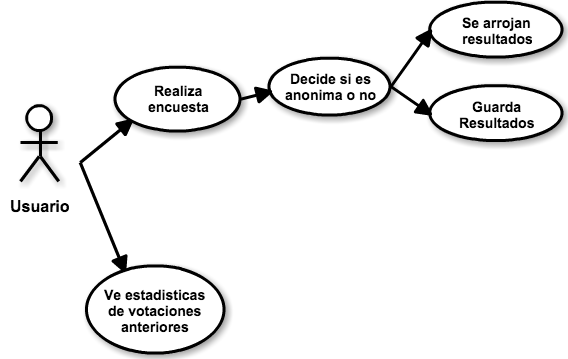
\includegraphics[width=0.8\linewidth]{UseCaseDiagram}
  \caption{Diagrama casos de uso.}
  \label{fig:sim2}
\end{figure}

\section{Marco Teórico}

Hemos decidido optar por la estrategia de desarrollo ágil SCRUM, en lugar de planificar y ejecutar de una sola vez el proyecto, dado que nos otorga un trabajo mas rápido y optimizado. 

Tomaremos en cuenta los requerimientos de la aplicación para designar las respectivas tareas a los miembros del grupo, por medio de reuniones periódicas veremos los objetivos o problemáticas a resolver (al ser reuniones periódicas, son soluciones cortas pero que traslapadas llegarán a una solución general del problema) y concluiremos en una reunión general en una fecha determinada, que será planificada dependiendo de los plazos fijados y nuevas instrucciones del cliente.

Para este periodo del proyecto, tenemos como tarea final dar a conocer las posibles soluciones que cada integrante cree que soluciona el problema, para llegar a un consenso general y comenzar el diseño y posterior desarrollo del proyecto.

Cuando llegamos al diseño de la plataforma decidimos ocupar diagramas de casos de uso y diagramas de flujo, que nos permiten una notación gráfica de cada caso de uso y por otra parte del algoritmo, respectivamente.

En cuanto a desarrollo lo que utilizamos fue el lenguaje C++ debido a que gracias a el podremos acceder a la biblioteca OpenCV, que es una biblioteca de libre acceso de visión artificial. La cual ocuparemos en las distintas tareas solicitadas ya sea reconocimiento facial, utilizar filtros para identificación de fondo, realizar el conteo, entre otras.


\section{Discusión}
La discusión básicamente fue mas orientada mas a la elección del proyecto a desarrollar que a las estrategias a utilizar. Se evaluaron factores de dificultad pero también áreas de interés de cada uno, eligiendo finalmente este proyecto de conteo automático de votos.

\section{Conclusión}
En conclusión, logramos concretizar los requerimientos que el cliente planteó para desarrollar el programa y resolver su problema, formalizamos también el enunciado, para entender lo que debíamos hacer y poder avanzar con las siguientes etapas dl proyecto.

Para todo esto, realizamos una evaluación de metodologías de trabajo y escogimos las más convenientes en base a las necesidades del trabajo.

El análisis y desarrollo se baso en la implementación de métodos y algoritmos correspondientes a las especificaciones pedidas, todo esto en una aplicación nativa en C++ con la biblioteca de OpenCV facilitando y optimizando el proceso de programación.

Finalmente las fechas de reuniones y metas a lograr en distintas fechas estan fijadas(estas son independientes y buscan cumplir con las fechas estipuladas) en una carta Gantt con la finalidad de entregar un proyecto integro al final de nuestro proceso de trabajo.

\newpage

\begin{figure*}[h]
  \centering
  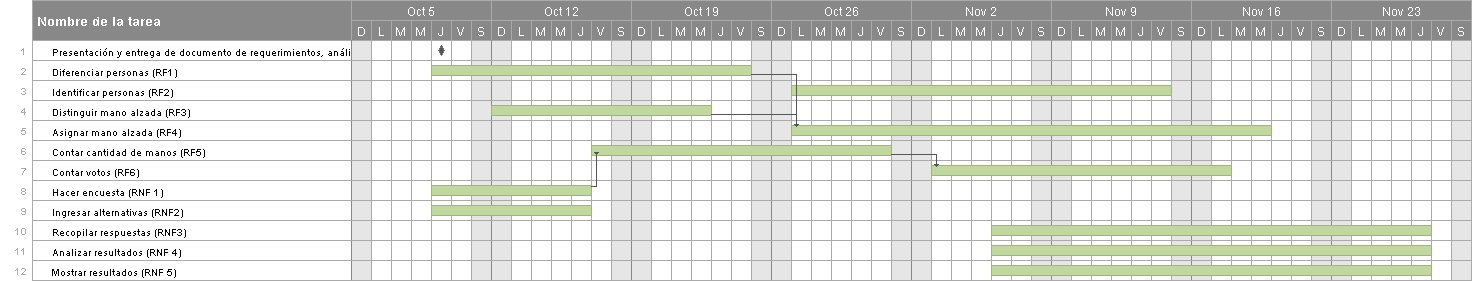
\includegraphics[width=1\linewidth]{Encuestamatic}
  \caption{Carta gantt.}
  \label{fig:sim2}
\end{figure*}
% Referencias

% can use a bibliography generated by BibTeX as a .bbl file
% BibTeX documentation can be easily obtained at:
% http://www.ctan.org/tex-archive/biblio/bibtex/contrib/doc/
% The IEEEtran BibTeX style support page is at:
% http://www.michaelshell.org/tex/ieeetran/bibtex/
%\bibliographystyle{IEEEtran}
% argument is your BibTeX string definitions and bibliography database(s)
%\bibliography{IEEEabrv,guia.bib}

% that's all folks
% don't panic!
\end{document}


